\documentclass[11pt,a4paper]{article}
\usepackage[T1]{fontenc}
\usepackage[utf8]{inputenc}
\usepackage{lmodern}
\usepackage[margin=25mm]{geometry}
\usepackage{amsmath,amssymb,amsthm,mathtools}
\usepackage{graphicx,booktabs,array}
\usepackage[section]{placeins}
\usepackage{microtype}
\usepackage{xcolor}
\usepackage[numbers,sort&compress]{natbib}
\usepackage{hyperref}
\hypersetup{colorlinks=true,linkcolor=blue!45!black,citecolor=blue!45!black,urlcolor=blue!45!black,
pdftitle={Equal-Circle Lens Geometry: Reparameterization, Identifiability, and Conditioning},
pdfauthor={Hilmir Frimann Halldorsson},pdfsubject={Draft v0.1.1; revised following project-internal proof review; final revision verification pending}}
\pagestyle{plain}
\makeatletter
\renewcommand{\@seccntformat}[1]{\makebox[2.5em][l]{\csname the#1\endcsname}}
\makeatother
\setlength{\emergencystretch}{2em}
\newtheorem{theorem}{Theorem}[section]
\newtheorem{proposition}[theorem]{Proposition}
\newtheorem{corollary}[theorem]{Corollary}
\theoremstyle{definition}
\newtheorem{example}[theorem]{Example}
\newtheorem{remark}[theorem]{Remark}
\newcommand{\dd}{\mathrm d}
\newcommand{\R}{\mathbb R}
\newcommand{\C}{\mathbb C}
\newcommand{\norm}[1]{\left\lVert#1\right\rVert}
\title{Equal-Circle Lens Geometry:\\
Reparameterization, Identifiability,\\and Conditioning}
\author{Hilmir Fr\'imann Halld\'orsson}
\date{9 October 2026\\[3pt]\small Draft v0.1.1 --- revised following project-internal proof review\\
\small Final revision verification pending}
\begin{document}
\maketitle
\begin{abstract}
For the filled intersection of two equal disks, perimeter and area are classical functions of the parent radius and a half-angle. We organize these functions as an inverse problem. Normalized perimeter, normalized area and a chosen nonnegative square-root gain are mutually recoverable shape coordinates, but they discard absolute scale. On the non-tangent equal-radius family, perimeter and area jointly determine the parent radius and separation up to rigid placement. A monotone restriction of the isoperimetric quotient gives a constructive proof and the exact admissible data image. Tangency loses parent-scale identifiability. Coincidence remains uniquely identifiable despite a singular endpoint Jacobian. Explicit asymptotics distinguish absolute error amplification from relative sensitivity: near tangency at fixed radius, the absolute area-error coefficient diverges, whereas the local relative half-angle sensitivity stays bounded. Near coincidence the half-angle inverse is sensitive even to relative errors. A short conditional linear-observation example separates geometry from an adopted response convention. Written proofs and reproducible high-precision illustrations are supplied; no physical measurement model or interpretation is inferred.
\end{abstract}

\section{Introduction and relation to prior work}
The intersection of two disks is a simple geometric object, but several different quantities can be called its profile: a set, its boundary length, its area, a normalized fraction, or a response derived from that fraction. The inverse questions differ accordingly. Does one number determine the shape? Does it determine the parent scale? Can two measured numbers determine both? Does exact uniqueness imply a stable reconstruction?

We answer these questions for two \emph{equal-radius} disks with nonnegative separation no larger than their diameter. The area formula follows from the classical circular-segment construction; standard accounts give both arc length and sector-minus-triangle area \citep{segment,intersection}. Our dimensionless statistic \(J=A/P^2\) is the familiar planar isoperimetric quotient divided by \(4\pi\) \citep{isoperimetric}. The contribution here is a self-contained synthesis of its restriction to this lens family, the resulting joint inverse and the endpoint sensitivity distinctions. We make no claim that the area formula, quotient, or elementary inverse arguments are first in the literature.

The presentation was motivated by reconstruction of historical Vesica and DMQPF source quantities \citep{vd,vpqw,dmqpfref}. Their notation combines different angle conventions and several inequivalent uses of the term profile. Those sources do not establish that normalized area is a normalized complex amplitude. We keep the historical correspondence in Appendix~\ref{app:history}; the geometric proofs require none of their physical assertions.

The central result is Theorem~\ref{thm:inverse}: every non-tangent lens in the declared family is determined, up to rigid placement, by \(P,A\). Corollary~\ref{cor:image} gives the complete data image. Section~\ref{sec:conditioning} then distinguishes an inverse from an already-known dimensionless \(J\) from an inverse that first forms \(J\) using \(P,A\). This distinction matters because conditioning depends on the input variables and error convention \citep{higham}. All error statements below are local mathematical sensitivities. They are neither a sensor model nor a uniform finite-noise guarantee.

\section{Lens geometry and measurements}\label{sec:geometry}
Choose a length unit. For \(r>0\) and \(0\le d\le 2r\), let
\begin{equation}\label{eq:disks}
 c_\pm=(\pm d/2,0),\qquad
 D_\pm=\{x\in\R^2:\norm{x-c_\pm}\le r\},\qquad
 L(r,d)=D_-\cap D_+ .
\end{equation}
The object \(L\) is a filled intersection. Let \(A\) be its planar area and \(P=\mathcal H^1(\partial L)\) its boundary length. Thus a coincident disk has its boundary counted once, and a tangent singleton has zero area and zero boundary length. Define the \emph{half-angle}
\begin{equation}\label{eq:theta}
 \theta=\arccos\!\left(\frac d{2r}\right)\in[0,\pi/2],
 \qquad d=2r\cos\theta .
\end{equation}
The parent radius and separation have units of length; angles in radians and all normalized quantities below are dimensionless. Figure~\ref{fig:geometry} shows the measured set and arcs.

\begin{table}[htbp]
\centering\small
\begin{tabular}{@{}p{.16\linewidth}p{.57\linewidth}p{.19\linewidth}@{}}
\toprule
Symbol & Meaning & Domain or units\\
\midrule
\(r,d\) & Common parent radius; center separation & \(r>0,\ 0\le d\le2r\)\\
\(\theta\) & Half of each boundary arc's central angle & \([0,\pi/2]\)\\
\(P,A\) & Boundary length; filled area & length; length\(^2\)\\
\(u,f\) & \(P/(2\pi r)\); \(A/(\pi r^2)\) & \([0,1]\)\\
\(G\) & Adopted nonnegative gain \(\sqrt f\) & \([0,1]\)\\
\(J\) & Scale-invariant ratio \(A/P^2\), \(P>0\) & \((0,1/(4\pi)]\)\\
\(\epsilon,K\) & \(\pi/2-\theta\); relative coefficient \(J/(\theta J')\) & Interior definitions\\
\bottomrule
\end{tabular}
\caption{Notation. The symbol \(\dd\) denotes a differential; the italic \(d\) denotes center separation.}
\end{table}

\begin{proposition}[Lens measurements]\label{prop:geometry}
For the domain in \eqref{eq:disks}--\eqref{eq:theta},
\begin{equation}\label{eq:PA}
 P=4r\theta,\qquad A=r^2(2\theta-\sin 2\theta).
\end{equation}
At \(d=0\) these give \(P=2\pi r,A=\pi r^2\); at \(d=2r\) they give \(P=A=0\).
\end{proposition}
\begin{proof}
First take \(0<d<2r\). The two intersection points have coordinates
\((0,\pm r\sin\theta)\). At either parent center the two radii to these points enclose the full angle \(2\theta\). The lens boundary consists of the arc of each parent circle contained in the other disk. These arcs meet only at the two intersection points, which do not affect the length sum. Each has length \(2r\theta\), giving \(P=4r\theta\).

One half of the lens is a circular segment (sector minus triangle): a sector of angle \(2\theta\), less the isosceles triangle between its two radii. The sector area is \(r^2\theta\), and the triangle area is \(r^2\sin(2\theta)/2\). Doubling the segment area gives \eqref{eq:PA}. At \(d=0\) the two limiting segments are complementary semicircles; their arcs cover the disk boundary once. At \(d=2r\) the intersection is a point. Directly evaluating the geometric measures at these endpoints agrees with the displayed formulas.
\end{proof}

\begin{figure}[htbp]
\centering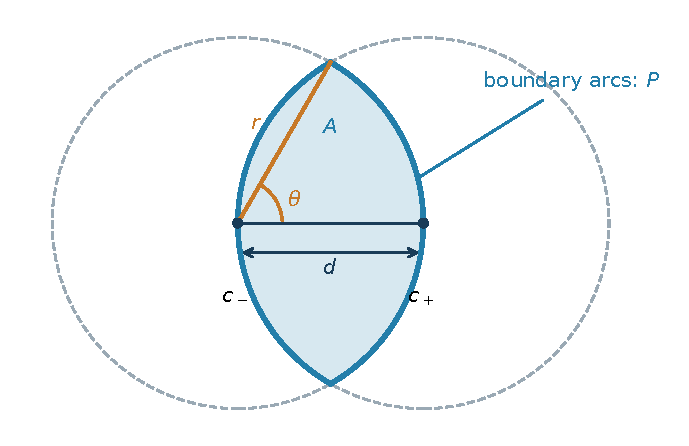
\includegraphics[width=.88\linewidth]{figures/01_geometry.pdf}
\caption{The filled lens for \(r=1,\theta=\pi/3,d=1\). Dashed parent circles define the construction; the two blue arcs are the measured boundary and the shading is the measured area. The angle marked at \(c_-\) is \(\theta\), half the full arc angle.}
\label{fig:geometry}
\end{figure}

When a source uses a full central angle \(\alpha\), its convention is \(\alpha=2\theta\). In particular, the center-on-circumference vesica has \(d=r\), hence \(\theta=\pi/3\). The example \(\theta=\pi/4\) instead has \(d=\sqrt2\,r\). Neither is selected by the inverse problem as a preferred constant. Equations~\eqref{eq:theta}--\eqref{eq:PA} are not definitions for \(d>2r\). One may separately assign zero measures to disjoint intersections, but that convention would identify many additional parent configurations and is not the present domain.

\section{Normalized shape coordinates}\label{sec:normalized}
Define
\begin{equation}\label{eq:normalized}
 u=\frac{P}{2\pi r},\qquad
 f=\frac{A}{\pi r^2},\qquad G=\sqrt f .
\end{equation}
The first two are geometric fractions. Calling \(G\) a response gain is an additional convention, used only in Section~\ref{sec:application}. Figure~\ref{fig:normalized} compares the three coordinates.

\begin{proposition}[Equivalent shape coordinates]\label{prop:normalized}
On the declared family,
\begin{equation}\label{eq:f}
 u=\frac{2\theta}{\pi},\qquad
 f=F(u):=u-\frac{\sin(\pi u)}{\pi}.
\end{equation}
The map \(F:[0,1]\to[0,1]\) is a strictly increasing bijection. Thus each of \(u,f,G\) determines \(d/r\), and none determines absolute radius or rigid placement. Near tangency, as \(u\downarrow0\),
\begin{equation}\label{eq:cubic}
 f=\frac{\pi^2}{6}u^3-\frac{\pi^4}{120}u^5+O(u^7),
 \qquad u\sim\left(\frac{6f}{\pi^2}\right)^{1/3}.
\end{equation}
\end{proposition}
\begin{proof}
Substitution of \eqref{eq:PA} in \eqref{eq:normalized} gives \eqref{eq:f}.
The function is continuous, with \(F(0)=0,F(1)=1\), and
\[
 F'(u)=1-\cos(\pi u).
\]
This derivative is positive for \(0<u\le1\). For any \(0\le a<b\le1\),
\(F(b)-F(a)=\int_a^b (1-\cos(\pi v))\,\dd v>0\).
Continuity and the endpoint values give surjectivity; strictness gives injectivity. The square root is also a bijection of \([0,1]\), with inverse squaring. Consequently each coordinate determines \(\theta=\pi u/2\) and \(d/r=2\cos\theta\).

For every \(\lambda>0\), scaling \((r,d)\) to \((\lambda r,\lambda d)\) preserves \(\theta,u,f,G\); translations and rotations preserve them as well. Thus these measurements cannot encode scale or placement. Finally, the Taylor series of \(\sin(\pi u)\) gives \eqref{eq:cubic}; inversion of its positive leading term gives the stated asymptotic equivalence.
\end{proof}

In particular,
\begin{equation}\label{eq:uf_sensitivity}
 \frac{\dd u}{\dd f}=\frac1{1-\cos(\pi u)}
 \sim\frac{2}{\pi^2u^2}\quad(u\downarrow0).
\end{equation}
This concerns inversion from an absolute error in \(f\); it does not assert identical sensitivity for every way of acquiring \(f\). Nor does mutual recoverability turn an area fraction into a boundary length or a complex state. For \(0<u<1\), \(f<u\), since \(\sin(\pi u)>0\).

\begin{figure}[htbp]
\centering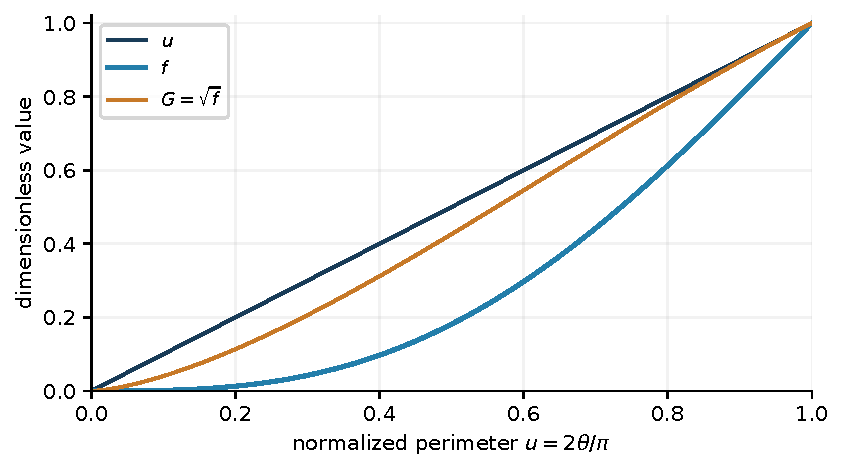
\includegraphics[width=.84\linewidth]{figures/02_normalized.pdf}
\caption{Normalized perimeter \(u\), area \(f\), and adopted gain \(G=\sqrt f\), on \(0\le u\le1\). Coincident endpoint values do not equate their quantity types. All curves are dimensionless and independent of \(r\).}
\label{fig:normalized}
\end{figure}

\section{Joint identifiability from perimeter and area}\label{sec:inverse}
Normalized measurements discard the parent scale. The unnormalized pair restores it except at tangency. For \(P>0\), introduce
\begin{equation}\label{eq:J}
 J(\theta)=\frac{A}{P^2}
 =\frac{2\theta-\sin2\theta}{16\theta^2}.
\end{equation}
The standard isoperimetric quotient is \(4\pi J\). We only need its monotonicity on this one-parameter shape family, not a characterization of arbitrary planar bodies. Figure~\ref{fig:J} shows its shape dependence and endpoint gap.

\begin{theorem}[Joint inverse]\label{thm:inverse}
For \(r>0\) and \(0<\theta\le\pi/2\), the pair \((P,A)\) uniquely determines \((r,d)\), hence the equal-radius lens and its parent disks up to rigid placement and exchange of the parent labels. The recovery order is
\begin{equation}\label{eq:inverse}
 J=A/P^2\ \longmapsto\ \theta\ \longmapsto\
 r=\frac{P}{4\theta}\ \longmapsto\ d=2r\cos\theta.
\end{equation}
\end{theorem}
\begin{proof}
Differentiating \eqref{eq:J} and simplifying with
\(\sin2\theta=2\sin\theta\cos\theta\) gives
\begin{equation}\label{eq:Jprime}
 J'(\theta)=
 \frac{\cos\theta(\sin\theta-\theta\cos\theta)}{4\theta^3}.
\end{equation}
Put \(h(\theta)=\sin\theta-\theta\cos\theta\). Since \(h(0)=0\) and
\(h'(\theta)=\theta\sin\theta>0\) on \((0,\pi/2)\), \(h\) is positive there. Also \(\cos\theta>0\), so \(J'>0\) throughout the interior. The numerator in \eqref{eq:J} is \(4\theta^3/3+O(\theta^5)\); hence \(J(\theta)\to0\) as \(\theta\downarrow0\). At the other endpoint, \(J(\pi/2)=1/(4\pi)\). Although its endpoint derivative is zero, \(J\) is strictly increasing on all of \((0,\pi/2]\): integrating its positive derivative over any nonempty interior subinterval establishes strictness even for an interval ending at \(\pi/2\).

Thus \(J\) uniquely identifies \(\theta\). The positive measured \(P\) then gives exactly one positive \(r\) in \eqref{eq:inverse}, and \eqref{eq:theta} gives exactly one \(d\). Two equal disks with that common radius and separation differ only by rigid placement or by exchanging their labels. This includes the coincident-disk endpoint.
\end{proof}

\begin{corollary}[Exact data image]\label{cor:image}
Among finite real data, the complete image of the declared family is
\begin{equation}\label{eq:image}
 \{(0,0)\}\ \cup\
 \left\{(P,A):P>0,\quad 0<A\le\frac{P^2}{4\pi}\right\}.
\end{equation}
Every pair in the second set has a unique reconstruction. The pair \((0,0)\) is compatible with every \(r>0\) at \(d=2r\).
\end{corollary}
\begin{proof}
Non-tangent lenses have positive \(P,A\), and Theorem~\ref{thm:inverse} gives \(0<J\le1/(4\pi)\), proving necessity. Conversely, any pair in the second set gives \(J\) in that interval. Continuity, strict increase, and the endpoint values \(J(0^+)=0\) and \(J(\pi/2)=1/(4\pi)\) established in the theorem's proof give a unique \(\theta\in(0,\pi/2]\); set \(r=P/(4\theta)>0\) and \(d=2r\cos\theta\). The constructed perimeter is \(P\), and its area is \(P^2J=A\). Finally, \eqref{eq:PA} at \(\theta=0\) gives \((0,0)\) for arbitrary positive \(r\).
\end{proof}

Thus positive perimeter with zero area, negative data, and \(A>P^2/(4\pi)\) are outside this exact model. A noisy observation may fall outside the image; the theorem supplies no clipping, projection or statistical fitting rule. At tangency, even though every filled lens is a singleton up to placement, the generating radius is not identifiable.

\begin{figure}[htbp]
\centering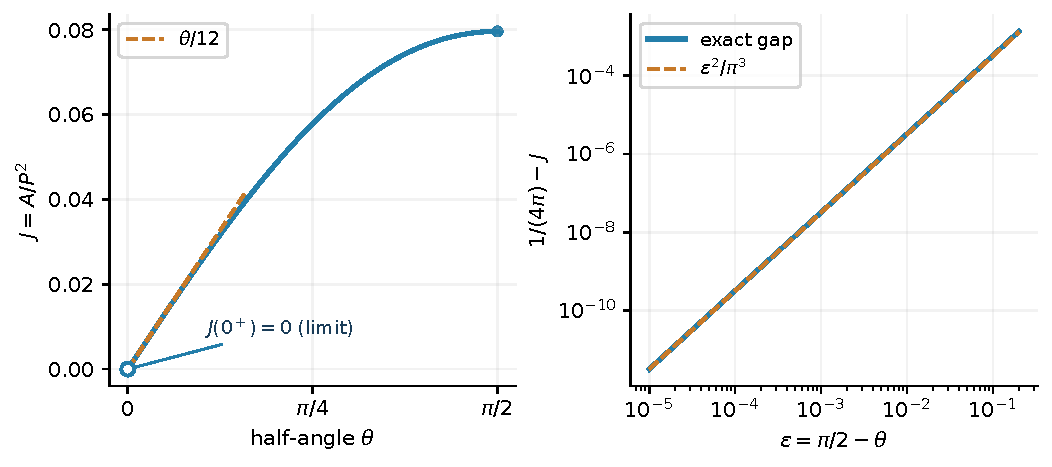
\includegraphics[width=\linewidth]{figures/03_shape_invariant.pdf}
\caption{Left: the strictly increasing \(J\), with the tangent asymptote \(J\sim\theta/12\) shown only near zero. The open tangent marker denotes \(\lim_{\theta\to0^+}J(\theta)=0\), not a value of \(A/P^2\) at \((P,A)=(0,0)\). Right: the coincident-endpoint gap against \(\epsilon=\pi/2-\theta>0\), with its quadratic asymptote. High-precision evaluation avoids cancellation in both small differences. Neither panel is a monotonicity proof.}
\label{fig:J}
\end{figure}

\begin{example}[Perimeter alone is insufficient]\label{ex:perimeter}
Take \((r_1,\theta_1)=(1/2,\pi/3)\) and
\((r_2,\theta_2)=(1/3,\pi/2)\). Then
\begin{align}
 P_1=P_2&=\frac{2\pi}{3},&
 A_1&=\frac{\pi}{6}-\frac{\sqrt3}{8},&
 A_2&=\frac{\pi}{9}.\label{eq:counterexample}
\end{align}
The areas differ: at fixed positive \(P\), the strict increase of \(J\) and \(\theta_1<\theta_2\) imply \(A_1<A_2\). The first object has \(d_1=1/2\); the second has \(d_2=0\). If \(r\) were known instead, \(P=4r\theta\) would already determine the shape. The ambiguity concerns unknown parent scale; Figure~\ref{fig:ambiguity} displays the two sets.
\end{example}

\begin{figure}[htbp]
\centering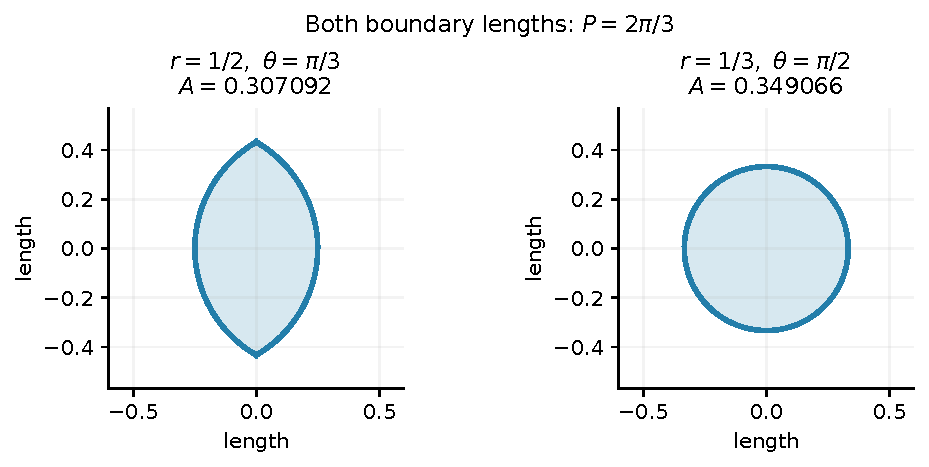
\includegraphics[width=.95\linewidth]{figures/04_equal_perimeter.pdf}
\caption{The two filled sets in Example~\ref{ex:perimeter}, using identical spatial scales and a common chosen length unit. Their perimeters agree, but their areas do not. Area values shown numerically are illustrations of the exact values in \eqref{eq:counterexample}.}
\label{fig:ambiguity}
\end{figure}

\section{Conditioning and endpoint error models}\label{sec:conditioning}
Identifiability is an exact-data statement. Conditioning asks how a selected inverse output responds to a specified perturbation of its inputs. We treat \(P,A\) as independent coordinates in the interior of \eqref{eq:image}. The notation \(\dd A,\dd P,\dd\theta\) denotes first-order differentials at a fixed interior point; it must not be read as an exact finite-error identity.

\subsection{Local differentials}
\begin{proposition}[Interior inverse and sensitivity]\label{prop:local}
For \(r>0,0<\theta<\pi/2\), the map \((r,\theta)\mapsto(P,A)\) has positive Jacobian determinant
\begin{equation}\label{eq:det}
 \det\frac{\partial(P,A)}{\partial(r,\theta)}
 =16r^2\cos\theta(\sin\theta-\theta\cos\theta)>0.
\end{equation}
The local shape inverse has differentials
\begin{align}
 \dd J&=\frac{\dd A}{P^2}-\frac{2A}{P^3}\dd P,
 & \dd\theta&=\frac{\dd J}{J'(\theta)},\label{eq:absolute}\\
 \frac{\dd J}{J}&=\frac{\dd A}{A}-2\frac{\dd P}{P},
 &\frac{\dd\theta}{\theta}
 &=K(\theta)\left(\frac{\dd A}{A}-2\frac{\dd P}{P}\right),
 \qquad K(\theta)=\frac{J(\theta)}{\theta J'(\theta)}>0.\label{eq:relative}
\end{align}
\end{proposition}
\begin{proof}
Direct differentiation of \eqref{eq:PA} gives
\[
 \frac{\partial(P,A)}{\partial(r,\theta)}
 =\begin{pmatrix}
 4\theta&4r\\
 2r(2\theta-\sin2\theta)&4r^2\sin^2\theta
 \end{pmatrix}.
\]
Its determinant equals
\(16r^2[\theta\sin^2\theta-\theta+\sin\theta\cos\theta]\),
which reduces to \eqref{eq:det}. Positivity follows from the same \(h\) argument used in Theorem~\ref{thm:inverse}. The inverse function theorem therefore applies in the interior. Differentiating \(J=A/P^2\) gives the first formula in \eqref{eq:absolute}; differentiating \(J(\theta)\) gives the second. Since \(P,A,J,\theta,J'\) are positive here, division by them yields \eqref{eq:relative}.
\end{proof}

For small absolute perturbations \(\Delta P,\Delta A\) at a fixed interior point, these formulas give the linear term in the inverse change, with a remainder of order \(O(\norm{(\Delta P,\Delta A)}^2)\) in fixed numerical units and locally admissible data. The remainder estimate is local and its constant need not remain bounded as the base point approaches an endpoint.

For example, if each input has small relative error bounded by \(\eta\), the linearized worst-case bound is
\begin{equation}\label{eq:firstorderbound}
 \frac{|\dd\theta|}{\theta}\le 3K(\theta)\eta .
\end{equation}
The factor \(3\) is the sum of the absolute coefficients \(1\) and \(2\) in \eqref{eq:relative}, not a claim that real errors attain those signs. Equation~\eqref{eq:firstorderbound} does not control a finite noise distribution, nor is it a bound on the omitted remainder.

\subsection{Tangency and coincidence}
\begin{corollary}[Endpoint asymptotics]\label{cor:endpoints}
At fixed \(r>0\), as \(\theta\downarrow0\),
\begin{align}
 J&=\frac{\theta}{12}-\frac{\theta^3}{60}
       +\frac{\theta^5}{630}+O(\theta^7),
 &J'&=\frac1{12}-\frac{\theta^2}{20}+O(\theta^4),\label{eq:Jtangent}\\
 \frac{\partial J}{\partial A}
 &=\frac1{16r^2\theta^2},
 &\frac{\partial J}{\partial P}&\longrightarrow-\frac1{24r},\label{eq:Jcoeff}\\
 \frac{\partial\theta}{\partial A}
 &\sim\frac3{4r^2\theta^2},
 &\frac{\partial\theta}{\partial P}&\longrightarrow-\frac1{2r},
 \qquad K(\theta)\longrightarrow1.\label{eq:thetacoeff}
\end{align}
These partial derivatives are taken in the measured \((P,A)\) coordinates, holding the other measurement fixed. Fixed \(r\) specifies only the family of base lenses used for the endpoint limit; these are not derivatives along the constrained curve \(r=\mathrm{constant}\). At the other endpoint, with \(\epsilon=\pi/2-\theta\downarrow0\),
\begin{equation}\label{eq:diskasymp}
 \frac1{4\pi}-J\sim\frac{\epsilon^2}{\pi^3},
 \qquad J'\sim\frac{2\epsilon}{\pi^3},
 \qquad K\sim\frac{\pi}{4\epsilon}.
\end{equation}
The Jacobian determinant has endpoint behavior
\begin{equation}\label{eq:detasymp}
 \det\frac{\partial(P,A)}{\partial(r,\theta)}
 \sim\frac{16}{3}r^2\theta^3\quad(\theta\downarrow0),
 \qquad
 \sim16r^2\epsilon\quad(\epsilon\downarrow0).
\end{equation}
\end{corollary}
\begin{proof}
The Taylor expansion
\[
 2\theta-\sin2\theta
 =\frac43\theta^3-\frac4{15}\theta^5
   +\frac8{315}\theta^7+O(\theta^9)
\]
inserted in \eqref{eq:J} yields \eqref{eq:Jtangent}; the analytic power series can be differentiated. Since \(P=4r\theta\), the area coefficient in \eqref{eq:absolute} is exactly \(1/(16r^2\theta^2)\). The perimeter coefficient is
\[
 -\frac{2A}{P^3}
 =-\frac{2\theta-\sin2\theta}{32r\theta^3}
 \longrightarrow-\frac1{24r}.
\]
Dividing both coefficients by \(J'\to1/12\) proves \eqref{eq:thetacoeff}, including the limit \(K=J/(\theta J')\to1\).

For coincidence, \(\cos\theta=\sin\epsilon\sim\epsilon\),
\(\sin\theta-\theta\cos\theta\to1\), and
\(4\theta^3\to\pi^3/2\). Equation~\eqref{eq:Jprime} gives
\(J'\sim2\epsilon/\pi^3\). Integrating this asymptotic from
\(\theta=\pi/2-\epsilon\) to \(\pi/2\) gives the gap
\(\epsilon^2/\pi^3\). Substitution in \(K\), using
\(J\to1/(4\pi)\) and \(\theta\to\pi/2\), proves the final expression in \eqref{eq:diskasymp}.

Finally, near tangency
\(\sin\theta-\theta\cos\theta=\theta^3/3+O(\theta^5)\)
and \(\cos\theta\to1\). Near coincidence the two factors tend respectively to \(1\) and \(\epsilon\). Substitution in \eqref{eq:det} proves \eqref{eq:detasymp}.
\end{proof}

The distinction is precise. Recovering \(\theta\) from an \emph{already-known} \(J\) has \(\dd\theta/\dd J\to12\) near tangency. Forming that \(J\) from measured \(P,A\) introduces the divergent absolute area coefficient in \eqref{eq:Jcoeff}. The absolute perimeter coefficient stays finite. In contrast, fixed small \emph{relative} errors in \(P,A\) give a bounded local relative half-angle coefficient as the base lens tends to tangency. These statements coexist because fixed relative area error requires absolute error to shrink with \(A\sim(4/3)r^2\theta^3\). No relative error in the zero endpoint area itself has been defined. Figures~\ref{fig:absolute} and~\ref{fig:relative} keep these error conventions separate.

\begin{figure}[htbp]
\centering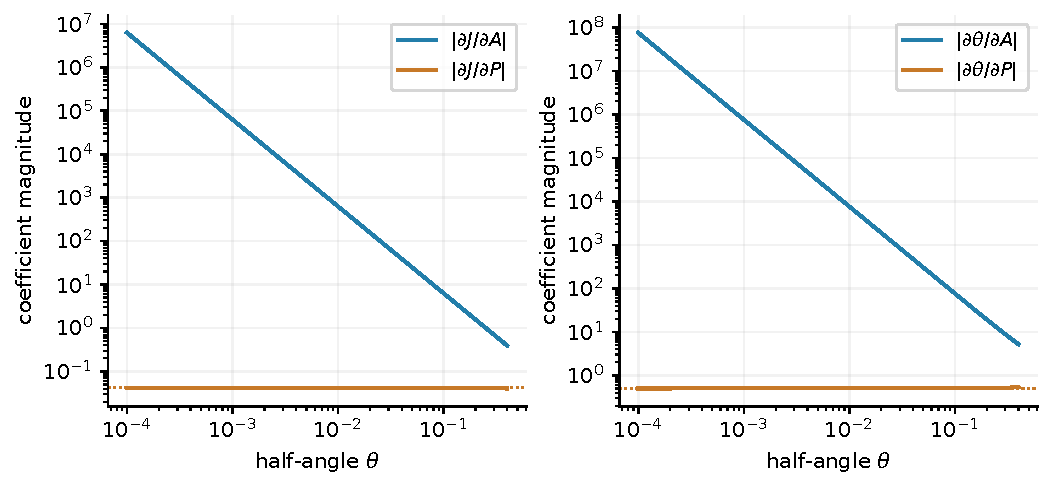
\includegraphics[width=\linewidth]{figures/05_absolute_sensitivity.pdf}
\caption{Absolute differential coefficients along the family with numerical radius \(r=1\) in a fixed length unit, for \(10^{-4}\le\theta\le0.4\). Left: forming \(J\) from \(P,A\). Right: recovering \(\theta\) from those inputs. Dotted horizontal lines show the finite magnitudes \(1/24\) and \(1/2\). Signs of the perimeter coefficients are negative. Area and perimeter coefficients have different dimensions; the plot illustrates endpoint behavior, not a unit-independent ranking of errors. The singular point \(\theta=0\) is excluded.}
\label{fig:absolute}
\end{figure}

\begin{figure}[htbp]
\centering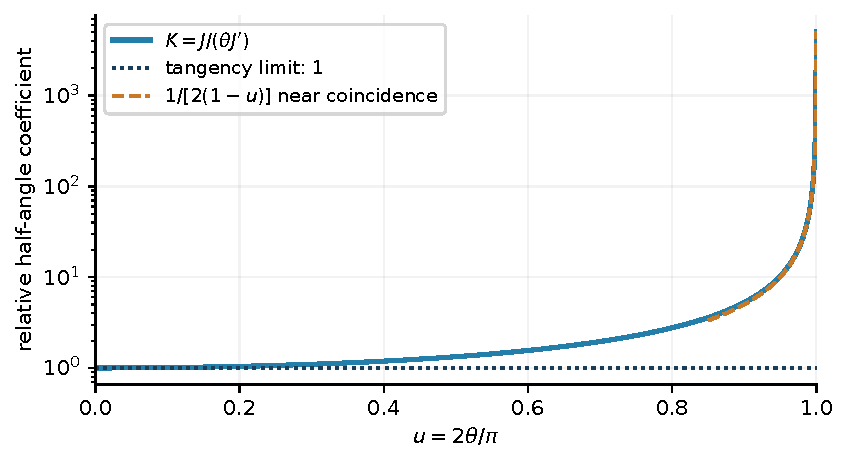
\includegraphics[width=.87\linewidth]{figures/06_relative_sensitivity.pdf}
\caption{The coefficient \(K\) in the local relative-error relation \eqref{eq:relative}, for \(0.001\le u\le0.9999\). It tends to \(1\) at tangency and diverges at coincidence. The dashed coincidence asymptote uses \(\epsilon=\pi(1-u)/2\). Endpoints are excluded from numerical evaluation; the finite tangent limit is an analytic statement.}
\label{fig:relative}
\end{figure}

Near coincidence \(\dd\theta/\dd J\sim\pi^3/(2\epsilon)\) diverges. More explicitly, on the admissible side,
\begin{equation}\label{eq:holder}
 \frac\pi2-\theta
 \sim \pi^{3/2}\sqrt{\frac1{4\pi}-J}.
\end{equation}
The endpoint inverse is therefore not locally Lipschitz in \(J\): the angle change divided by the \(J\) change diverges. This is consistent with global uniqueness at the coincident disk. A zero Jacobian at a boundary point rules out the interior inverse-function argument there; it does not produce a second solution.

These sensitivity results concern \(\theta\). For other outputs the calculation changes. In the interior,
\[
 \frac{\dd r}{r}=\frac{\dd P}{P}-\frac{\dd\theta}{\theta},
 \qquad
 \frac{\dd d}{d}=\frac{\dd r}{r}-\tan\theta\,\dd\theta
 \quad(d>0).
\]
The latter has no relative-error meaning at \(d=0\). We do not transfer the half-angle bounds to separation, radius or a later observable without their own coefficients and input assumptions.

\section{A declared response and observation example}\label{sec:application}
This section is a conditional application of the quantity distinctions. Adopt \(G=\sqrt f\) and supply an independent complex vector \(\xi\in\C^2\), together with the unit vector
\[
 f_0=\frac{1}{\sqrt3}(1,1,1)^{\mathsf T}\in\C^3.
\]
The reconciled preparation convention \citep[Section 6]{dmqpfref} is
\begin{equation}\label{eq:prep}
 \Psi_0=\sqrt f\,(\xi\otimes f_0)\in\C^6 .
\end{equation}
This equation is an adopted map with side inputs, not a geometric derivation of a complex state.

\begin{proposition}[Conditional scalar readout]\label{prop:observation}
Let both \(\xi\in\C^2\) and the prescribed linear map \(B:\C^6\to\C^k\) be fixed independently of \(f\). Identify \(\C^2\otimes\C^3\cong\C^6\) by
\[
 \xi=(\xi_0,\xi_1)^T,\qquad
 (\xi\otimes f_0)_{3h+j}=\xi_h(f_0)_j,
 \quad h=0,1,\quad j=0,1,2.
\]
This is the \(\xi\)-major (source helicity-major) convention of \citet[Section 6]{dmqpfref}; no physical helicity interpretation is implied. The matrix of \(B\) uses this same ordered input basis. With Euclidean complex norms,
\begin{equation}\label{eq:intensity}
 \norm{\Psi_0}^2=f\norm{\xi}^2.
\end{equation}
More generally,
\begin{equation}\label{eq:readout}
 I=\norm{B\Psi_0}^2=m f,\qquad
 m=\norm{B(\xi\otimes f_0)}^2\ge0.
\end{equation}
Known \(m>0\) permits scalar recovery \(f=I/m\) on the admitted range \(0\le I\le m\). Unknown \(m\) generally confounds that recovery, and \(m=0\) erases all information about \(f\).
\end{proposition}
\begin{proof}
The tensor product has entries \(\xi_h(f_0)_j\), so
\[
 \norm{\xi\otimes f_0}^2
 =\sum_{h=0}^1\sum_{j=0}^2|\xi_h|^2|(f_0)_j|^2
 =\norm{\xi}^2\norm{f_0}^2=\norm{\xi}^2.
\]
Scaling by \(\sqrt f\) proves \eqref{eq:intensity}. Linearity of the prescribed \(B\), followed by the same norm scaling, proves \eqref{eq:readout}. If \(m>0\) is known, division is valid. If it is unknown, for example \((f,m)=(1/4,4)\) and \((1/2,2)\) both give \(I=1\); different admitted fractions cannot then be distinguished from that observation alone. If \(m=0\), every fraction gives \(I=0\).
\end{proof}

The symbol \(B\) is an explicit abstract observation convention, not a claim that this general map is a new runtime feature. A particular transfer or readout would require its source vector, operator and branch inputs to be specified. Equations~\eqref{eq:prep}--\eqref{eq:readout} neither recover these inputs from the lens nor recover the parent radius from \(f\). Complex phases, scale and a physical interpretation are not created by the norm identity.

\section{Scope and conclusions}\label{sec:limits}
Within the equal-radius family, normalized perimeter and normalized area are exact alternative shape coordinates; their square-root transform is another nonnegative coordinate. Absolute scale is lost by normalization and restored by joint positive perimeter--area data. The exact data image and reconstruction order make both the uniqueness claim and its tangency exception explicit.

Stability depends on how those data are supplied. Near tangency, \(J\) as an independent input has a finite angle derivative, but constructing \(J\) from absolute area measurements introduces unbounded amplification. Under fixed small relative input errors the local relative half-angle coefficient instead remains bounded. At coincidence the angle inverse is singular on the admissible side even though the disk is uniquely determined. These distinctions should precede any proposed measurement or response interpretation.

The family restriction is essential. We have not identified unequal parent radii, arbitrary convex sets, noisy out-of-model data, or an experimental error distribution. The bounded literature search supports classical attribution and methods positioning, not a comprehensive priority claim. The historical unknowns listed below do not alter the geometric proof chain. A future physical model would require independent premises and is outside this draft.

\appendix
\section{Bounded historical correspondence}\label{app:history}
The following table distinguishes the source quantities used for motivation. It is a correspondence record, not an endorsement of the historical titles' physical claims.

\begin{table}[htbp]
\centering\small
\begin{tabular}{@{}>{\raggedright\arraybackslash}p{.22\linewidth}>{\raggedright\arraybackslash}p{.7\linewidth}@{}}
\toprule
Quantity & Source status and consequence\\
\midrule
Filled lens, \(P,A\) & VD, p.~1, Eqs.~(1)--(3), gives the lens geometry; VPQW, p.~2, Section 3, uses a full central angle. These are reconciled by \(\alpha=2\theta\), not by identifying different measures.\\[4pt]
Normalized \(u,f\) & Dimensionless boundary and area fractions. Their exact bijection is \eqref{eq:f}; they are unequal in the interior.\\[4pt]
Gain \(G=\sqrt f\) & Adopted in the reconciled preparation map. No recovered source equality of normalized amplitude and normalized area is used.\\[4pt]
VPQW separation weight & VPQW, p.~2, Section 4, Eq.~(3), gives a proportional Gaussian weight \(\exp[-d^2/(4r^2)]\). At \(d=2r\) this factor is \(e^{-1}>0\), whereas \(f=0\); it is not the normalized lens area.\\[4pt]
DMQPF variants & The February source, p.~1, Section 2, combines a perimeter factor multiplicatively with other factors. Later additive definitions are separate records; common names do not give equality.\\[4pt]
Delay and selected constants & A delay table compatible with a fitted construction does not recover its simulation producer. The historical selection of literal \(.618\) remains unresolved. Neither supplies a premise for the present inverse theorem.\\
\bottomrule
\end{tabular}
\caption{Relevant source distinctions. Historical sources are \citet{vd,vpqw,dmqpf}; the consolidated definitions and limitations are in \citet[Sections 1--7]{dmqpfref}.}
\end{table}

The final conditioning interpretation follows the later reconciliation
\citep[Section 3]{toroidaddendum} and accepted refinements
\citep[R6]{refinements}. An earlier unqualified characterization of near-tangency recovery as well conditioned is insufficient: it omits the operation of forming \(J\) from measured \(P,A\). Section~\ref{sec:conditioning} supplies the error-model distinction directly rather than requiring the reader to reconstruct the review history.

Unresolved historical meanings retained here are the absence of a recovered area--amplitude equality, the lack of identified delay-table producer provenance, and the rationale for selecting literal \(.618\). February and later additive DMQPF are inequivalent definitions, not a gap to be closed by merging them. None is assigned a dark-matter, gravity, quantum-hardware or transport interpretation in this paper.

\section{Reproducibility and review status}\label{app:repro}
The accompanying review package contains the editable manuscript and bibliography, six vector figures, their generation script and numerical data, one isolated checker and machine-readable results. The checker uses symbolic differentiation and limits, independent area quadrature, exact counterexamples and high-precision scalar reconstruction. The paper-only inverse uses bracketing of \(J\), admits the coincident endpoint explicitly and rejects data outside \eqref{eq:image}; it is not a new public API or a statistical fitting algorithm.

Figures use the displayed formulas and high precision where subtraction near an endpoint would lose digits. Sampling a positive derivative does not prove monotonicity, and a collection of algebra checks is not a theorem count. The written proofs above provide the mathematical arguments. The scripts do not import or execute project runtime or historical simulations. Exact file identities and commands accompany the package; hashes identify artifacts, not mathematical truth.

\paragraph{AI assistance and authorship.}
Hilmir Fr\'imann Halld\'orsson is the sole named author. OpenAI Codex assisted with source organization, targeted reference checking, drafting, mathematical derivations, standalone symbolic/numerical checks, figure generation, revision and typesetting. GPT and Claude contributed to underlying derivations, source reconciliation and project-internal manuscript review.

The v0.1 manuscript received GPT and Claude reviews, which found no proof errors in the stated domains and requested minor clarifications, metadata and presentation edits. The reconciled disposition was pass with minor revisions. Claude had participated in the underlying project derivations; the fresh manuscript-level check was within that shared project. These AI-assisted reviews were project-internal, not external peer review.

Draft v0.1.1 implements the bounded reconciled changes. Final verification of this revised edition remains pending; no reviewer approval of its final bytes or publication authorization is claimed. No affiliation, funding or new license is asserted.

\bibliographystyle{plainnat}
\bibliography{references}
\end{document}
